\documentclass[17pt, c]{beamer}
\setbeamertemplate{caption}[numbered]

\usepackage[brazil]{babel}

\title{Template de exemplo para Apresentações}
\subtitle{Com Beamer}
\date{\today}
\institute[DCC]{DCC -- Departamento de Ciência da Computação}
\author[Author et al]{João Autor da Silva}

% para matemática
\usepackage{amsmath,amssymb,mathtools}

% Probably load as late as possible
% Other options are
% - engine=pdflatex to compile in pdfLaTeX (with different fonts),
% - mathshape=rm to use serif font for math,
% - mathsahpe=custom to not set any math font (so that you can define your own math fonts)
\usetheme[mathshape=rm]{fineUFLA}
%\setmonofont{Bitstream Vera Sans Mono}[Scale=.9]

\newif\ifabnt
\abnttrue
\ifabnt
\usepackage{setspace}
\usepackage[alf, abnt-etal-list=3, abnt-emphasize=bf]{abntex2cite}
\fi


\begin{document}

\inserttitlepage

\inserttoc{Sumário}

\section{Introdução}
\insertsectionpage

\begin{frame}{Exemplo Slide de Texto}
Lorem ipsum dolor sit amet, consectetur adipiscing elit. Sed eu odio at purus varius elementum. Aliquam ut libero ac nulla posuere mattis eget sit amet libero. Sed tempor finibus tincidunt. Fusce commodo, felis id accumsan porttitor, libero velit auctor elit, ut laoreet purus augue ut mi \cite{Martins2000,NBR6023:2000}.
Maecenas at ultrices metus, nec auctor risus. Donec in ipsum malesuada, elementum nunc id, pharetra sem. Vestibulum rutrum nec risus ut congue. Aliquam a pharetra felis. Fusce laoreet porttitor magna, id consectetur tellus sodales eu. Mauris posuere in nibh id facilisis \cite{Moura1998}.
Fusce lacinia sodales lorem, vitae dignissim nunc. Etiam lobortis dui at lorem sodales ullamcorper a ut nisl. Fusce in odio eget ante laoreet feugiat facilisis et lacus. Proin orci massa, suscipit in sem quis, pulvinar aliquet diam \cite{Silva2005,Lamport1994}.
\end{frame}


\section{Trabalhos Relacionados}
\insertsectionpage
\begin{frame}{Utilizando Equações}
	Phasellus nec accumsan lorem. Pellentesque fermentum risus urna, quis tempor dolor consectetur non. Sed commodo enim dui, sed varius quam hendrerit eleifend. Sed feugiat faucibus facilisis. Fusce a ullamcorper leo, sed vehicula eros. Proin lobortis pellentesque mi ut lobortis. Aliquam bibendum turpis velit, non fermentum eros aliquam volutpat. Fusce nec mollis lacus:
	\begin{equation}
		f_a(x) = \sum_{i = 1}^{x}\frac{a^{i + 1}}{i} \pi
	\end{equation}
\end{frame}


\section{Metodologia}
\insertsectionpage
\begin{frame}{Duas colunas}
\begin{columns}
	\column{0.5\textwidth}
		Phasellus nec accumsan lorem. Pellentesque fermentum risus urna, quis tempor dolor consectetur non. Sed commodo enim dui, sed varius quam hendrerit eleifend. Sed feugiat faucibus facilisis. Fusce a ullamcorper leo, sed vehicula eros. Proin lobortis pellentesque mi ut lobortis. Aliquam bibendum turpis velit, non fermentum eros aliquam volutpat. Fusce nec mollis lacus
	\column{0.5\textwidth}
		Phasellus nec accumsan lorem. Pellentesque fermentum risus urna, quis tempor dolor consectetur non. Sed commodo enim dui, sed varius quam hendrerit eleifend. Sed feugiat faucibus facilisis. Fusce a ullamcorper leo, sed vehicula eros. Proin lobortis pellentesque mi ut lobortis. Aliquam bibendum turpis velit, non fermentum eros aliquam volutpat. Fusce nec mollis lacus
\end{columns}
\end{frame}


\section{Resultados}
\insertsectionpage
\begin{frame}{Imagem}
\begin{columns}
	\column{0.5\textwidth}
	Phasellus nec accumsan lorem. Pellentesque fermentum risus urna, quis tempor dolor consectetur non. Sed commodo enim dui, sed varius quam hendrerit eleifend. Sed feugiat faucibus facilisis. Fusce a ullamcorper leo, sed vehicula eros. Proin lobortis pellentesque mi ut lobortis.
	
	\column{0.5\textwidth}
	\begin{figure}
		\vspace{-1cm}
		\caption{Imagem de exemplo}
		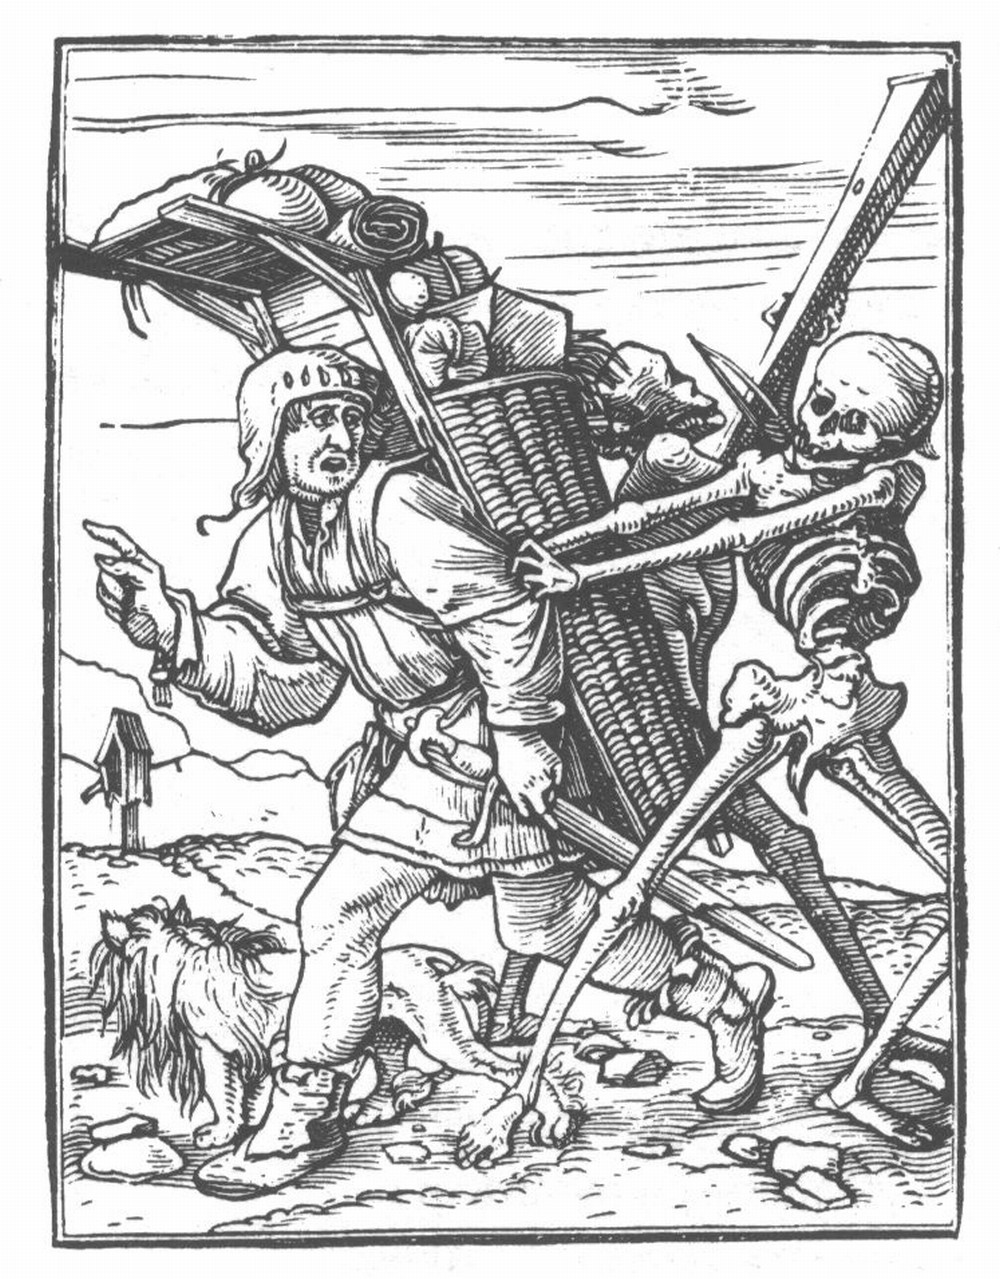
\includegraphics[scale=0.225]{imgs/Holbein_Danse_Macabre}\\
		Fonte: domínio público
	\end{figure}%
\end{columns}
\end{frame}


\section{Conclusão}
\insertsectionpage
\begin{frame}{Utilizando blocos}
	\begin{block}{Definição}
		Lorem ipsum dolor sit amet, consectetur adipiscing elit. Sed eu odio at purus varius elementum. Aliquam ut libero ac nulla posuere mattis eget sit amet libero. Sed tempor finibus tincidunt! \cite{UFLA2015}
	\end{block}
	\begin{exampleblock}{Exemplo}
		Sed eu odio at purus varius elementum. Aliquam ut libero ac nulla posuere mattis eget sit amet libero. Sed tempor finibus tincidunt!
	\end{exampleblock}
	\begin{alertblock}{Alerta}
		Lorem ipsum dolor sit amet, consectetur adipiscing elit! \cite{Franca2001} 
	\end{alertblock}
\end{frame}


\section{Referências}
\setbeamertemplate{headline}[UFLA-frametitle-only]
\begin{frame}[t, allowframebreaks]{Referências}
	\ifabnt
		\bibliographystyle{abntex2-alf}%
		\citeoption{abnt-etal-text=it}%
		\citeoption{abnt-etal-cite=3}%
		\citeoption{abnt-missing-year=sd}%
		\citeoption{abnt-nbr10520=1988}%
		\vspace{-0.7cm}
	\else
		\bibliographystyle{siam}
	\fi
		\bibliography{refbib}
\end{frame}

\insertendpage

\end{document}